%% \documentclass[twoside]{report}
\documentclass[a4paper]{report}


\usepackage[sc]{mathpazo}
\usepackage[T1]{fontenc}
\usepackage[utf8]{inputenc}
\usepackage[frenchb]{babel}
\linespread{1.05}
\usepackage{microtype}

%% \usepackage[hmarginratio=1:1,top=32mm,columnsep=20pt]{geometry}
%% \usepackage{multicol}
\usepackage[hang, small,labelfont=bf,up,textfont=it,up]{caption}
\usepackage[top=3cm, bottom=4cm, left=3cm, right=2.5cm]{geometry} 
\usepackage{booktabs}
\usepackage{float} 
\usepackage{hyperref}

\usepackage{graphicx}

\usepackage{lettrine}
\usepackage{paralist}
\usepackage{setspace}

\usepackage{abstract}
\renewcommand{\abstractnamefont}{\normalfont\bfseries}
\renewcommand{\abstracttextfont}{\normalfont\small\itshape}

\usepackage{titlesec}
%% \renewcommand\thesection{\Roman{section}}
%% \renewcommand\thesubsection{\Roman{subsection}}
\titleformat{\chapter}[hang]{\bf\huge}{\thechapter}{2pc}{} 
\titleformat{\section}[block]{\large}{\textbf\thesection.}{1em}{\textbf}
\titleformat{\subsection}[block]{\large}{\thesubsection.}{1em}{}





%----------------------------------------------------------------------------------------
%% TITLE SECTION
%----------------------------------------------------------------------------------------

\title{\vspace{+0cm}\fontsize{24pt}{10pt}\selectfont\textbf{Monitoring du noyau Linux sur une architecture NUMA}}

\author{
\large
\textsc{Kévin Gallardo, Eric Lombardet, Pierre-Yves Péneau}\\[2mm] 
\normalsize Université Pierre et Marie Curie - Jussieu - Paris VI
\vspace{-5mm}
}
\date{}

%----------------------------------------------------------------------------------------
%% HEADER STYLE
%----------------------------------------------------------------------------------------
\usepackage{fancyhdr}
\pagestyle{fancy}
\fancyhead{} 
\fancyfoot{}
%% \fancyhead[C]{Monitoring du noyau Linux sur une architecture NUMA $\bullet$ \author}
%% \fancyfoot{\thepage}


%----------------------------------------------------------------------------------------
\begin{document}
  \maketitle
  \newpage

  \tableofcontents
  \newpage

  \setcounter{page}{0}
  \thispagestyle{empty}
  \begin{abstract}
    \centering
    \noindent L’essor de l’informatique en nuage a permis aux administrations et entreprises
de stocker d’énormes jeux de données. Aujourd’hui, l’un des goulots
d’étranglement majeurs pour les performances de traitement de ces données est le
système d’exploitation de chaque machine. Les systèmes actuels ne peuvent pas
gérer efficacement les applications intensives en données car ils ne disposent
pas d’une vue unifiée des ressources utilisées, ce qui les empêche de déterminer
des stratégies efficaces pour le placement des tâches/données sur les ressources
matérielles. Une meilleure gestion des ressources permettrait une forte
réduction du nombre de machines nécessaires aux traitements des données.

L’implémentation de sondes dans le noyau Linux permettrait d'identifier les
ressources physiques et logicielles les plus sollicitées par les processus. Les
informations remontées par ces sondes peuvent ensuite permettre de commencer à
définir des stratégies de placement des tâches et des données prenant en compte
à la fois la topologie de la machine et l’utilisation effectives des ressources
par les tâches.

  \end{abstract}
  \newpage
  
  \begin{onehalfspace}
  \chapter{Introduction}

  \lettrine[nindent=0em,lines=3]{L} es systèmes multicoeurs modernes sont
  maintenant basés sur l'architecture NUMA (Non Uniforme Memory Access). Avec un
  système NUMA, les coeurs des processeurs sont regroupés en noeuds. Chaque
  noeud possède un contrôleur mémoire et est interconnecté avec les autres
  noeuds de la machine.

  \begin{figure}[H]
    \centering
    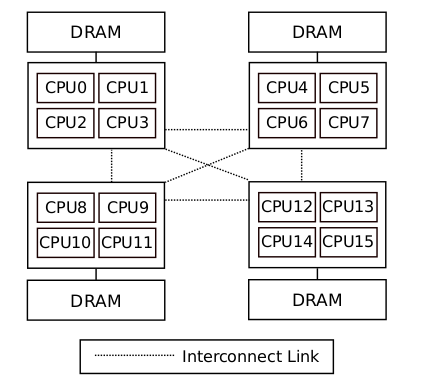
\includegraphics[scale=0.35]{img/numa_arch.png}
    \caption{Un système NUMA avec 4 noeuds et 4 coeurs par noeud}
    \label{f:numa_arch}
  \end{figure}

  Du fait des temps d'accès mémoire non uniforme, tout le défi des systèmes
  tournant sur cette architecture est la répartition des données et des
  traitements. En effet, la principale cause de latence n'est pas due au
  \textbf{temps de traitement des données}, mais au \textbf{temps d'accès aux
    données}. Ces accès coûtent entre 10\% et 40\% de temps supplémentaire par
  rapport aux accès locaux.\cite{Lepers2014} Dans une configuration idéale,
  chaque coeur irait chercher ce dont il a besoin dans la mémoire contrôlée par
  le noeud dans lequel il se situe. Ainsi, les demandes d'accès distant seraient
  réduites à néant, et il n'y aurait aucune latence due aux échanges entre les
  noeuds. Nous allons voir que cet idéal est très difficile, voire impossible à
  obtenir. Néanmoins, il est possible de s'en approcher, en mettant au point des
  algorithmes de répartitions de plus en plus efficaces. La création de ces
  algorithmes nécessite une connaissance approfondie du noyau: comment gère-t-il
  la création des threads, où sont-ils placés, quelles sont les pages mémoires
  accédées le plus souvent, par quels noeuds sont-elles contrôlées\ldots C'est
  en collectant un maximum de renseignements sur ces différents points (et de
  nombreux autres) que l'on pourra être en mesure d'affiner les solutions de
  répartition de charge. Cette étape de monitoring sera le sujet principal de ce
  projet de master. Nous allons devoir lire et comprendre le fonctionnement à
  très bas niveau du noyau, puis le modifier en utilisant divers outils de
  gestions d'évènements avec des bibliothèques comme IBS\footnote{Instruction
    Base Sampling, une technologie développée par AMD uniquement sur les
    processeurs Opteron} afin de préparer l'étape de réflexion pour la création
  d'algorithmes.

  \subsection{Étude du contexte}

  \lettrine[nindent=0em,lines=3]{L}e but de se projet sera dans un premier temps
  de mettre en place une infrastructure de compilation, de test et d'exécution
  d'un noyau Linux. La seconde partie du projet sera de comprendre comment
  fonctionne le noyau Linux au niveau de la mémoire, notamment pour la gestion
  des pages (emplacement, taille), et au niveau des processeurs pour le
  placement des threads et me parallélisme. Ensuite, il faudra se plonger dans
  la lecture du code et sa modification aux endroits adéquats en utilisant des
  technologies comme IBS où les hardware counters pour obtenir des informations
  précises sur la gestion des points évoqués ci-dessus. Enfin, pour tester ce
  noyau avec nos modifications, nous utiliserons la machine virtuelle et gdb
  pour le débugage.
  %% TODO: changer débugage par autre chose

  \subsubsection{Infrastructure}
    Dans cette partie, nous allons détailler l'infrastructure dont nous
    disposons et celle que nous avons mise en place pour ce projet. Notre avons
    à notre disposition une machine AMD Opteron 6172 composée de quatre
    processeurs à douze coeurs chacun cadencés à 2,1GHz et répartis en 8 noeuds
    avec 32G de mémoire vive. L'architecture des noeuds est la
    suivante\footnote{Source: \textit{Improving performance on NUMA systems},
      Baptiste Lepers}:

    %% TODO: vérifier l'archi à la main (méga chaud et méga long)

    %% node   0   1   2   3   4   5   6   7 
    %%   0:  10  16  16  22  16  22  16  22 
    %%   1:  16  10  16  22  22  16  22  16 
    %%   2:  16  16  10  16  16  16  16  22 
    %%   3:  22  22  16  10  16  16  22  16 
    %%   4:  16  22  16  16  10  16  16  16 
    %%   5:  22  16  16  16  16  10  22  22 
    %%   6:  16  22  16  22  16  22  10  16 
    %%   7:  22  16  22  16  16  22  16  10

    \begin{figure}[H]
      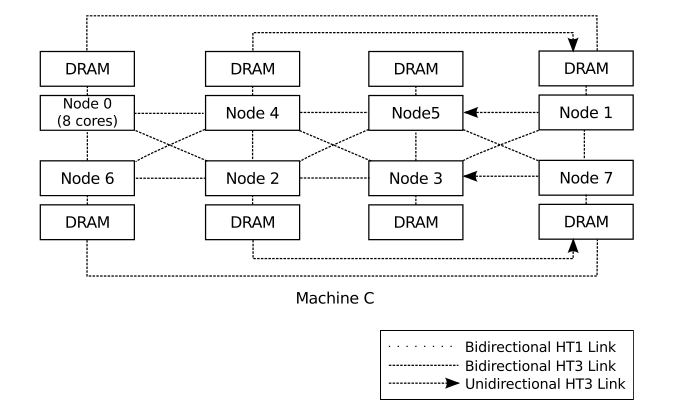
\includegraphics[scale=0.4]{img/numa_topology.png}
      \caption{Topologie de la machine 6172}
      \label{f:numa_topology}
    \end{figure}

    Sur cette machine, nous avons utilisé l'hyperviseur qemu, avec son extension
    kvm pour afin d'optimiser l'émulation. Afin d'améliorer encore plus cette
    dernière, nous avons utilisé le logiciel virt-manager qui détecte
    automatiquement la configuration matérielle de machine hôte et configure la
    machine virtuelle en conséquence. Cette configuration est à notre avis très
    réaliste puisqu'elle est capable d'activer/désactiver des options CPU comme
    la gestion d'IBS où l'hypervision. Un des autres avantage de virt-manager
    est que l'on peut sauvegarder la configuration dans un fichier, et pouvoir
    ainsi l'exporter facilement.

    Nous avons installé une machine virtuelle classique (Debian GNU/Linux), qui
    nous permettra par la suite de fournir à notre noyau compilé une
    architecture de base pour se lancer. En effet, la compilation du noyau se
    fera directement sur l'Opteron, mais le lancement et les tests se feront via
    l'hyperviseur. Afin que le noyau puisse se lancer et avoir une base, nous
    avons installé une première VM, donc nous récupérerons la configuration du
    noyau pour la compilation.

    Cette étape ne fût pas sans difficulté. Nous avons passé plus d'une semaine
    dessus, alors qu'il s'agit simplement d'installer une machine
    virtuelle. Malheureusement, l'université à eu des problèmes de réseux, et
    notamment de ssh la semaine six, le serveur a lui du être mis à jour, il y a
    eu des souçis de compatibilité de version de logiciels entre nos machines et
    le serveur, des souçis de virtualisation de matériel\ldots


  \subsubsection{Fonctionnement de la mémoire}
  
    TODO


  \subsubsection{Placement des threads}
    TODO


  \newpage
\begin{thebibliography}{99}

  \bibitem[1]{Lepers2014} Baptiste Lepers, Phd. Thesis (2014).
    \newblock \textit{Improving performances on NUMA systems architecture.}
  
  \bibitem[2]{Holistic2013} Mohammad Dashti, Alexandra Fedorova, Justin Funston,
    Fabien Gaud, Renaud Lachaize, Baptiste Lepers, Vivien Quéma, and Mark
    Roth.
    \newblock \textit{Traffic Managment: A holistic Approach to Memory
      Placement on NUMA Systems}.
    \newblock Architectural Support for Programming Languages and Operating
    Systems (ASPLOS), Houston, USA, March 2013.
  \bibitem[3]{BKDG10th} 2005–2013 Advanced Micro Devices, Inc.
  	\newblock \textit{BIOS and Kernel Developer’s Guide (BKDG) For AMD Family 10h Processors}
  	Rev 3.62  - January 11, 2013
  \bibitem[4]{CacheHierarchy}Pat Conway, Nathan Kalyanasundharam, Gregg Donley, Kevin Lepak, Bill Hughes, Advanced Micro Devices, Inc.
  	\newblock{CACHE HIERARCHY AND MEMORY SUBSYSTEM OF THE AMD OPTERON PROCESSOR}
  \bibitem[5]{BasicPerformanceMesurements}Paul J. Drongowski
  	\newblock \textit{Basic Performance Measurements for AMD AthlonTM 64, AMD OpteronTM and AMD PhenomTM Processors}
  	Advanced Micro Devices, Inc. Boston Design Center, 25 September 2008


\end{thebibliography}

  \end{onehalfspace}

\end{document}
